\begin{center}
    \tikzstyle{w} = [rectangle, rounded corners, minimum width=2cm, text width=4cm, minimum height=1cm, text centered, draw=black, fill=white]
    \tikzstyle{cu} = [rectangle, rounded corners, minimum width=2cm, text width=10cm, minimum height=1cm, text centered, draw=black, fill=white]
    \tikzstyle{p} = [rectangle, rounded corners, minimum width=2cm, text width=2cm, minimum height=1cm, text centered, draw=black, fill=white]
    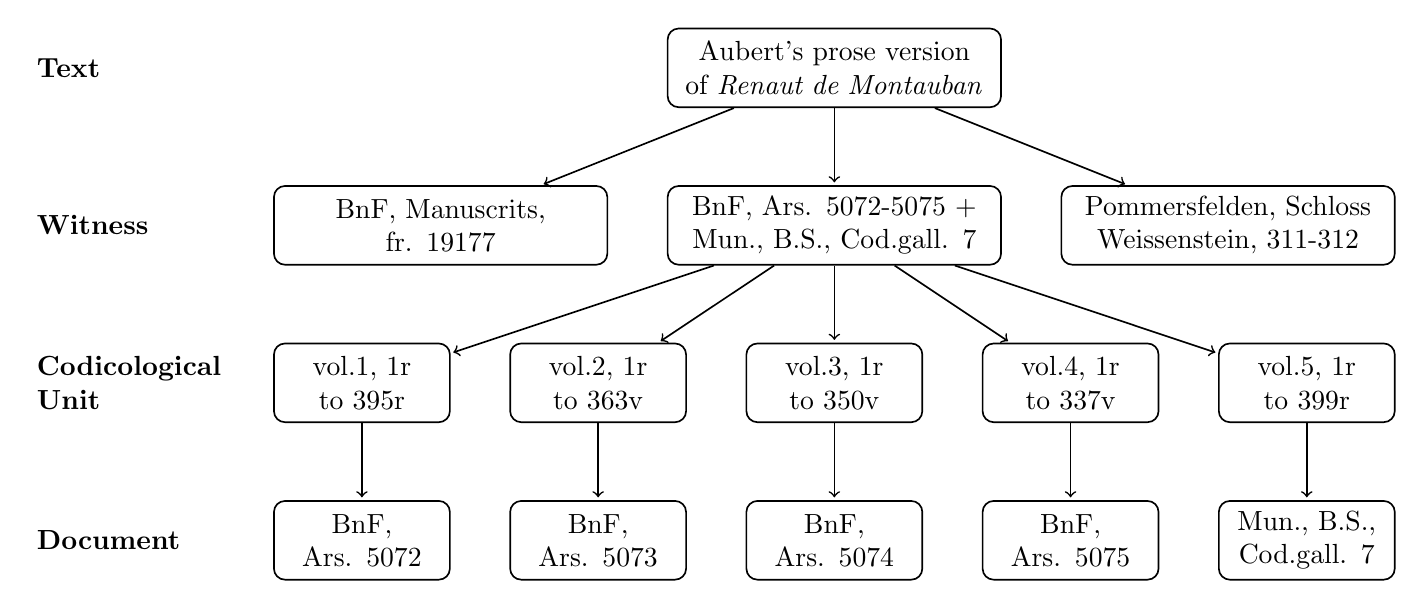
\begin{tikzpicture}[->,shorten >=1pt,auto,node distance=2cm,semithick]
        \node[w] (b) {BnF, Manuscrits, fr. 19177};
        \node[w] (a) [right of=b, xshift=3cm] {BnF, Ars. 5072-5075 + Mun., B.S., Cod.gall. 7};
        \node[w] (c) [right of=a, xshift=3cm] {Pommersfelden, Schloss Weissenstein, 311-312};
        \node(an) [left=3cm, text width=2cm] at (b){\textbf{Witness}};
        \node[w] (t) [above of=a] {Aubert's prose version of \textit{Renaut de Montauban}};
        \node(tn) [left=8cm, text width=2cm] at (t){\textbf{Text}};
        \node[p] (pt3) [below of=a] {vol.3, 1r to 350v};
        \node[p] (pt2) [left of=pt3, xshift=-1cm] {vol.2, 1r to 363v};
        \node[p] (pt1) [left of=pt2, xshift=-1cm] {vol.1, 1r to 395r};
        \node[p] (pt4) [right of=pt3, xshift=1cm] {vol.4, 1r to 337v};
        \node[p] (pt5) [right of=pt4, xshift=1cm] {vol.5, 1r to 399r};
        \node(pn) [left=2cm, text width=2cm] at (pt1){\textbf{Codicological Unit}};
        \draw (t) -> (a);
        \draw (t) -> (b);
        \draw (t) -> (c);
        \draw (a) -> (pt1);
        \draw (a) -> (pt2);
        \draw (a) -> (pt3);
        \draw (a) -> (pt4);
        \draw (a) -> (pt5);
        \node[p] (pt1d) [below of=pt1] {BnF, Ars. 5072}; \draw (pt1) -> (pt1d);
        \node(dn) [left=1cm, text width=3cm] at (pt1d){\textbf{Document}};
        \node[p] (pt2d) [below of=pt2] {BnF, Ars. 5073}; \draw (pt2) -> (pt2d);
        \node[p] (pt3d) [below of=pt3] {BnF, Ars. 5074}; \draw (pt3) -> (pt3d);
        \node[p] (pt4d) [below of=pt4] {BnF, Ars. 5075}; \draw (pt4) -> (pt4d);
        \node[p] (pt5d) [below of=pt5] {Mun., B.S., Cod.gall. 7}; \draw (pt5) -> (pt5d);
    \end{tikzpicture}
\end{center}